\documentclass{report}
%%%%%%%%%%%%%% macros.tex %%%%%%%%%%%%%%
% Place your custom macros here, if any.

%%%%%%%%%%%%%% letterfonts.tex %%%%%%%%%%%%%%
% Place your font setup here, if any.

%%%%%%%%%%%%%% preamble.tex %%%%%%%%%%%%%%
\usepackage[T1]{fontenc}
\usepackage{lmodern}
\usepackage{etoolbox}
\usepackage{pdfpages}
\usepackage{transparent}
\usepackage[utf8]{inputenc}
\usepackage[english]{babel}

% Page Setup
\usepackage[tmargin=2cm, rmargin=0.5in, lmargin=0.5in, bmargin=80pt, footskip=.2in]{geometry}

% Mathematics
\usepackage{amsmath,amsfonts,amsthm,amssymb,mathtools}
\usepackage{xfrac}
\usepackage[makeroom]{cancel}
\usepackage{enumitem}
\usepackage{nameref}
\usepackage{multicol,array}
\usepackage{tikz-cd}
\usepackage[ruled,vlined,linesnumbered]{algorithm2e}

% Colors
\usepackage[dvipsnames]{xcolor}
\definecolor{myg}{RGB}{56, 140, 70}
\definecolor{myb}{RGB}{45, 111, 177}
\definecolor{myr}{RGB}{199, 68, 64}
% Define more colors here...

% Hyperlinks
\usepackage{bookmark}
\usepackage{hyperref}
\hypersetup{
    pdftitle={Assignment},
    colorlinks=true, linkcolor=doc!90,
    bookmarksnumbered=true,
    bookmarksopen=true
}

% Figures and Graphics
\usepackage{import}
\usepackage{svg}
\newcommand{\incfig}[1]{%
    \def\svgwidth{\columnwidth}
    \import{./figures/}{#1.pdf_tex}
}

% Text-related
\usepackage{blindtext}
\usepackage{fontsize}
\changefontsize[14]{14}
\setlength{\parindent}{0pt}

% Theorems and Definitions
\usepackage{amsthm}
\renewcommand\qedsymbol{$\blacksquare$}

% Define a new theorem style
\newtheoremstyle{mytheoremstyle}% name
  {}% Space above
  {}% Space below
  {\sffamily}% Body font
  {}% Indent amount
  {\bfseries}% Theorem head font
  {.}% Punctuation after theorem head
  {.5em}% Space after theorem head
  {}% Theorem head spec (can be left empty, meaning ‘normal’)

% Apply the new theorem style to theorem-like environments
\theoremstyle{mytheoremstyle}
\newtheorem{theorem}{Theorem}[section]
\newtheorem{definition}{Definition}[section]
\newtheorem{corollary}{Corollary}[section]
\newtheorem{lemma}{Lemma}[section]
\newtheorem{axiom}{Axiom}[section]

% tcolorbox Setup
\usepackage[most,many,breakable]{tcolorbox}

% Define custom tcolorbox environments here...

%================================
% EXAMPLE BOX
%================================
\newtcbtheorem[definition]{Example}{Example}
{%
    colback = myexamplebg,
    breakable,
    colframe = myexamplefr,
    coltitle = myexampleti,
    boxrule = 1pt,
    sharp corners,
    detach title,
    before upper=\tcbtitle\par\smallskip,
    fonttitle = \bfseries,
    description font = \mdseries,
    separator sign none,
    description delimiters parenthesis,
}
{ex}

%================================
% Solution BOX
%================================
\makeatletter
\newtcolorbox{solution}{enhanced,
	breakable,
	colback=white,
	colframe=myg!80!black,
	attach boxed title to top left={yshift*=-\tcboxedtitleheight},
	title=Solution,
	boxed title size=title,
	boxed title style={%
			sharp corners,
			rounded corners=northwest,
			colback=tcbcolframe,
			boxrule=0pt,
		},
	underlay boxed title={%
			\path[fill=tcbcolframe] (title.south west)--(title.south east)
			to[out=0, in=180] ([xshift=5mm]title.east)--
			(title.center-|frame.east)
			[rounded corners=\kvtcb@arc] |-
			(frame.north) -| cycle;
		},
}
\makeatother

%================================
% Question BOX
%================================
\makeatletter
\newtcbtheorem{question}{Question}{enhanced,
	breakable,
	colback=white,
	colframe=myb!80!black,
	attach boxed title to top left={yshift*=-\tcboxedtitleheight},
	fonttitle=\bfseries,
	title={#2},
	boxed title size=title,
	boxed title style={%
			sharp corners,
			rounded corners=northwest,
			colback=tcbcolframe,
			boxrule=0pt,
		},
	underlay boxed title={%
			\path[fill=tcbcolframe] (title.south west)--(title.south east)
			to[out=0, in=180] ([xshift=5mm]title.east)--
			(title.center-|frame.east)
			[rounded corners=\kvtcb@arc] |-
			(frame.north) -| cycle;
		},
	#1
}{def}
\makeatother
\makeatletter
\newtcbtheorem{qstion}{Question}{enhanced,
    breakable,
    colback=white,
    colframe=mygr,
    attach boxed title to top left={yshift*=-\tcboxedtitleheight},
    fonttitle=\bfseries,
    title={#2},
    boxed title size=title,
    boxed title style={%
        sharp corners,
        rounded corners=northwest,
        colback=tcbcolframe,
        boxrule=0pt,
    },
    underlay boxed title={%
        \path[fill=tcbcolframe] (title.south west)--(title.south east)
        to[out=0, in=180] ([xshift=5mm]title.east)--
        (title.center-|frame.east)
        [rounded corners=\kvtcb@arc] |-
        (frame.north) -| cycle;
    },
    #1
}{def}
\makeatother

%%%%%%%%%%%%%%%%%%%%%%%%%%%%%%%%%%%%%%%%%%%
% TABLE OF CONTENTS
%%%%%%%%%%%%%%%%%%%%%%%%%%%%%%%%%%%%%%%%%%%
\usepackage{tikz}
\definecolor{doc}{RGB}{0,60,110}
\usepackage{titletoc}
\contentsmargin{0cm}
\titlecontents{chapter}[14pc]
{\addvspace{30pt}%
	\begin{tikzpicture}[remember picture, overlay]%
		\draw[fill=doc!60,draw=doc!60] (-7,-.1) rectangle (-0.9,.5);%
		\pgftext[left,x=-4.5cm,y=0.2cm]{\color{white}\Large\sc\bfseries Chapter\ \thecontentslabel};%
	\end{tikzpicture}\color{doc!60}\large\sc\bfseries}%
{}
{}
{\;\titlerule\;\large\sc\bfseries Page \thecontentspage
	\begin{tikzpicture}[remember picture, overlay]
		\draw[fill=doc!60,draw=doc!60] (2pt,0) rectangle (4,0.1pt);
	\end{tikzpicture}}%
\titlecontents{section}[3.7pc]
{\addvspace{2pt}}
{\contentslabel[\thecontentslabel]{2pc}}
{}
{\hfill\small \thecontentspage}
[]
\titlecontents*{subsection}[3.7pc]
{\addvspace{-1pt}\small}
{}
{}
{\ --- \small\thecontentspage}
[ \textbullet\ ][]

\makeatletter
\renewcommand{\tableofcontents}{
	\chapter*{%
	  \vspace*{-20\p@}%
	  \begin{tikzpicture}[remember picture, overlay]%
		  \pgftext[right,x=15cm,y=0.2cm]{\color{doc!60}\Huge\sc\bfseries \contentsname};%
		  \draw[fill=doc!60,draw=doc!60] (13,-.75) rectangle (20,1);%
		  \clip (13,-.75) rectangle (20,1);
		  \pgftext[right,x=15cm,y=0.2cm]{\color{white}\Huge\sc\bfseries \contentsname};%
	  \end{tikzpicture}}%
	\@starttoc{toc}}
\makeatother

\newcommand{\liff}{\llap{$\iff$}}
\newcommand{\rap}[1]{\rrap{\text{ (#1)}}}
\newcommand{\red}[1]{\textcolor{red}{#1}}
\newcommand{\blue}[1]{\textcolor{blue}{#1}}
\newcommand{\vi}[1]{\textcolor{violet}{#1}}
\newcommand{\teal}[1]{\textcolor{teal}{#1}}
\newcommand{\tCaC}{\text{ \CaC }}
\newcommand{\CaC}{\red{CaC} }
\newcommand{\As}[1]{Assume \red{#1}}
\newcommand{\vdone}{\vi{\text{ (done) }}}
\newcommand{\bdone}{\blue{\text{ (done) }}}
\newcommand{\tdone}{\teal{\text{ (done) }}}
\newcommand{\set}[1]{\{ #1 \}}
\newcommand{\inS}{\in S}
\newcommand{\inF}{\in\F}
\newcommand{\inE}{\in E}
\newcommand{\inA}{\in A}
\newcommand{\inB}{\in B}
\newcommand{\inC}{\in C}
\newcommand{\inU}{\in U}

\newcommand{\C}{\mathbb{C}}	
\renewcommand{\H}{\mathbb{H}}
\newcommand{\F}{\mathbb{F}}
\newcommand{\N}{\mathbb{N}}
\newcommand{\Q}{\mathbb{Q}}
\newcommand{\R}{\mathbb{R}}
\newcommand{\Z}{\mathbb{Z}}
\renewcommand{\P}{\mathbb{P}}
\renewcommand{\S}{\mathbb{S}}
\newcommand{\A}{\mathbb{A}}
\newcommand{\RP}{\R P}


\title{\Huge{NCKU 112.2}\\
Miscellaneous Facts}
\author{\huge{Eric Liu}}
\date{}
\begin{document}
\maketitle
\newpage% or \cleardoublepage
% \pdfbookmark[<level>]{<title>}{<dest>}
\pdfbookmark[section]{\contentsname}{toc}
\tableofcontents
\pagebreak

\chapter{General Topology}
\section{Directed Sets}
\begin{axiom}
\label{1.1.1}
\textbf{(Axioms in Order Theory)} Given an relation $(X,\leq )$, and suppose  $x,y,z \in X$. 
\begin{enumerate}[label=(\alph*)]
  \item $x\leq x$ (Reflexive)
  \item $x\leq y\leq z \implies x\leq z$ (Transitive)
  \item $x\leq y\text{ and }y\leq x\implies x=y$ (Antisymmetric)
  \item $x\leq y\text{ or }y\leq x$ (Connected)
  \item $\forall x,y \in X, \exists z\in X, x\leq z\text{ and }y\leq z$ (Directed)
\end{enumerate}
We say $(X,\leq )$ form a 
\begin{enumerate}[label=(\alph*)]
  \item \red{total order} if it is reflexive, transitive, antisymmetric and connected. 
  \item \red{partial order} if it is reflexive, transitive and  antisymmetric. 
  \item \red{preorder} if it is reflexive and transitive.
  \item \red{directed set} if it is reflexive, transitive and directed. 
\end{enumerate}
\end{axiom}
\begin{theorem}
\label{1.1.2}
\textbf{(Why is it called Preorder)} Given a preorder $(X,\leq )$, the relation $\sim$ defined by 
\begin{align*}
x\sim y \iff x\leq y\text{ and }y\leq x
\end{align*}
is an equivalence relation and if we define $\leq^e$ on the equivalence class by 
\begin{align*}
\exists x \in A, y \in B, x\leq y \implies A\leq^e B
\end{align*}
Then $\leq^e$ is a partial order. Moreover, if the preorder $\leq $ is directed, then $\leq ^e$ is also directed.
\end{theorem}
\begin{proof}
We first show \vi{$\sim$ is an equivalence relation}. Because preoder is reflexive, we see 
\begin{align*}
\forall x\in X, x\leq x\text{ which implies }\forall x \in X, x \sim x
\end{align*}
For symmetry, it is easy to see 
\begin{align*}
x\sim y \implies x\leq y\text{ and }y\leq x\implies y\sim x
\end{align*}
For transitive, see 
\begin{align*}
  x\sim y \text{ and } y\sim z&\implies x\leq y \text{ and }y \leq x \text{ and }y\leq z \text{ and }z \leq y \\
&\implies x\leq z\text{ and } z\leq x\implies x\sim z \vdone
\end{align*}
We now show \blue{$\leq^e$ is a partial order}. Reflexive property and Transitive property of $\leq^e$ follow from that of $\leq $. Suppose $A\leq^e B$ and $B\leq^e A$, where $x_1,x_2\in A,y_1,y_2\in B$ satisfy $x_1\leq y_1$ and $y_2\leq x_2$. Because $x_1,x_2 \in A$ and $y_1,y_2\in B$, we have 
\begin{align*}
x_1\leq x_2\text{ and }x_2\leq x_1\text{ and }y_1\leq y_2\text{ and }y_2\leq y_1
\end{align*}
Then because $\leq $ satisfy transitive, we have 
\begin{align*}
\begin{cases}
  x_2\leq x_1\leq y_1 \implies x_2\leq y_1\\
  y_1\leq y_2\leq x_2 \implies y_1\leq x_2
\end{cases}
\end{align*}
This tell us 
\begin{align*}
x_2 \sim y_1
\end{align*}
which implies $A=B$, thus proving  $\leq^e$ is antisymmetirc. $\bdone$\\

Lastly, we show  \vi{$\leq $ is directed$\implies \leq ^e$ is directed}. Let $A,B$ be two arbitrary equivalence class. We wish to find an equivalence class $T$ such that 
\begin{align*}
A\leq^e T \text{ and } B\leq^e T
\end{align*}
Let $a,b$ respectively be an arbitrary element of $A,B$. Because  $\leq $ is directed, we know there exists $c\in X$ such that 
\begin{align*}
a\leq c\text{ and }b\leq c
\end{align*}
We immediately see 
\begin{align*}
A\leq^e [c] \text{ and } B\leq^e [c] \vdone
\end{align*}
\end{proof}
\begin{corollary}
\label{1.1.3}
\textbf{(Chunk Structure of Preorder)} Given two equivalence class $A,B$, we have
 \begin{align*}
A\leq^e B \implies \forall x\in A,y \in B, x\leq y
\end{align*}
\end{corollary}
\begin{proof}
Because $A\leq ^e B$, we know 
\begin{align*}
\exists x_0\in A,y_0\in B, x_0\leq y_0
\end{align*}
Then by definition of $\sim$, we have
\begin{align*}
x \leq x_0\leq y_0\leq y
\end{align*}
This give us 
\begin{align*}
x\leq y
\end{align*}
\end{proof}
\begin{definition}
\label{1.1.4}
\textbf{(Definition of Maximal element in Preorder)} Let $(I,\leq )$ be a preorder. We say $m\in I$ is a maximal element if 
\begin{align*}
\forall y\in I, m\leq y\implies y\leq m
\end{align*}
\end{definition}
\begin{theorem}
\label{1.1.5}
\textbf{(In Preorder, Maximal element form an Equivalence class)} Let $(I,\leq )$ be a preorder, and $m \in  I$ be a maximal element. Then 
\begin{align*} 
\forall x\in [m], x\text{ is a maximal element }
\end{align*}
\end{theorem}
\begin{proof}
Arbitrarily pick an element $x$ in $[m]$. Suppose 
\begin{align*}
x\leq y 
\end{align*}
By definition of $\sim$, we have 
\begin{align*}
m\leq x\leq y
\end{align*}
Thus $m\leq y$. Then because $m$ is maximal, we know $y\leq m$. This now give us 
\begin{align*}
y\leq m\leq x
\end{align*}
\end{proof}
\begin{mdframed}
Notice that in partially ordered set, where anti-symmetric property is true, the definition of maximal element $m \in I$ falls into 
\begin{align*}
\forall y \in I, m \leq y \implies y=m
\end{align*}
\end{mdframed}
\begin{definition}
\label{1.1.6}
\textbf{(Definition of Greatest element in Preorder)} Let  $(I,\leq )$ be a preorder. We say $x \in I$ is a greatest element if 
\begin{align*}
\forall y\in I, y\leq x
\end{align*}
\end{definition}
\begin{theorem}
\label{1.1.7}
\textbf{(In Directed Set, Maximal element is the Greatest)} Suppose $(I,\leq )$ is a directed set. 
 \begin{align*}
x\in I\text{ is a maximal element }\implies x\in I\text{ is the greatest element }
\end{align*}
\end{theorem}
\begin{proof}
Arbitrarily pick an element $y\in I$. Because  $I$ is directed, we see there exists  an element $z$ such that 
 \begin{align*}
y\leq z\text{ and }x\leq z
\end{align*}
Then because $x$ is maximal, we know 
\begin{align*}
y\leq z\leq x
\end{align*}
This shows 
\begin{align*}
y\leq x
\end{align*}
\end{proof}
\begin{theorem}
\label{1.1.8}
\textbf{(Sufficient Condition for Preorder to become Directed)} 
\begin{align*}
  (I,\leq )\text{ is a preorder and has a greatest element }x\implies I\text{ is a directed set }
\end{align*}
\end{theorem}
\begin{proof}
Given arbitrary two element $y,z \in I$, we see $y\leq x$ and $z\leq x$. 
\end{proof}
\begin{mdframed}
\begin{Example}{\textbf{(Partial Order that is Directed)}}{}
\begin{align*}
X=\set{a,b,c}\text{ and }a\leq c \text{ and } b \leq c
\end{align*}
\end{Example}
\begin{Example}{\textbf{(Partial Order that is Not Directed)}}{}
\begin{align*}
X=\set{a,b,c}\text{ and }a\leq b\text{ and }a\leq c
\end{align*}
\end{Example}
\begin{Example}{\textbf{(Partial Order that is Directed)}}{}
\begin{align*}
  X=\Z^+_0&\text{ and }\forall x,y \in\N, x\leq y\iff y-x |2 \text{ and }x\leq y\\
&\text{ and }\forall x \in\N, x\leq 0
\end{align*}
\end{Example}
\begin{Example}{\textbf{(Partial Order that is not Directed)}}{}
\begin{align*}
X=\N\text{ and }\forall x,y\inn, x\leq y\iff  y-x |2\text{ and }x\leq y
\end{align*}
\end{Example}
\begin{Example}{\textbf{(Directed Set that is not Partially Ordered)}}{}
\begin{align*}
  X=\set{a,b,c}&\text{ and }a\leq b\text{ and }b\leq a\\
&\text{ and }a\leq c\text{ and }b\leq c
\end{align*}
\end{Example}
\begin{Example}{\textbf{(Preorder that is Neither Directed nor Partially Ordered)}}{}
\begin{align*}
  X=\set{a,b,c,d}&\text{ and }a\leq b\text{ and }b\leq a\\
&\text{ and }a\leq c\text{ and }b\leq c\\
&\text{ and }a\leq d\text{ and }b\leq d
\end{align*}
\end{Example}
\begin{Example}{\textbf{(Directed Sets)}}{}
\begin{align*}
  X\text{ is a metric space and }x\leq y\iff  d(y,x_0)\leq  d(x,x_0) \text{ where $x_0$ is a fixed point in $X$ } 
\end{align*}
Notice that this directed set is generally not antisymmetric, meaning it generally isn't a partial order. Also, notice that $x_0$ is the greatest element. Also, this order is connected, meaning if we take equivalence class on it, it become a total order.\\

Lastly, notice that if we remove $x_0$,  $X$ can still be directed, say if $X=\R^2$ and $x_0$ is the origin.
\end{Example}
\begin{Example}{\textbf{(Directed Sets)}}{}
  \vspace{1cm}
Suppose $X,Y$ are both directed sets. We see $X\times Y$ is a directed set if we define 
\begin{align*}
  (x,y)\leq (a,b)\iff  x\leq a\text{ and }y\leq b  
\end{align*}
\end{Example}
\begin{Example}{\textbf{(Partial Order)}}{}
  \vspace{1cm}
Every collection of sets is a partial order if we define 
\begin{align*}
A\leq B \iff  A\subseteq B
\end{align*}
Also, every collection of sets form a partial order if we define 
\begin{align*}
A\leq B \iff  A \supseteq B
\end{align*}
\end{Example}
\begin{Example}{\textbf{(Directed Sets)}}{}
  \vspace{1cm}
Suppose $(X,\tau)$ is a topological space and  $x \in X$. Then all of $\tau$, neighborhoods of $x$ and open neighborhoods of  $x$ form directed sets under $\subseteq $, since $X$ is open.\\

Also, $\tau$, neighborhoods of $x$ and open neighborhoods of  $x$ form directed sets under  $\supseteq$, because intersection of two open set is again an open set and intersection of two neighborhood is again a neighborhood.
\end{Example}
\includegraphics[height=10cm,width=10cm]{drawing.pdf}
\end{mdframed}
\begin{definition}
\label{1.1.9}
\textbf{(Definition of Cofinal)} Given a directed set $\mathcal{D}$, a subset $\mathcal{D}'\subseteq \mathcal{D}$ is called cofinal if 
\begin{align*}
\forall d \in \mathcal{D},\exists e\in \mathcal{D}', d\leq e 
\end{align*}
\end{definition}
\begin{theorem}
\label{1.1.10}
\textbf{(Cofinal Subset is a Directed Set with Original Order)} Given a directed set $\mathcal{D}$
 \begin{align*}
 \mathcal{D}'\subseteq \mathcal{D}\text{ is cofinal }\implies \mathcal{D}'\text{ is a directed set }
 \end{align*}
\end{theorem}
\begin{proof}
Arbitrarily pick two $a,b \in \mathcal{D}'$. Because $\mathcal{D}\ni a,b$ is directed, we know 
\begin{align*}
\exists c \in \mathcal{D}, a\leq c \text{ and } b\leq c
\end{align*}
Then because $\mathcal{D}'$ is cofinal in $\mathcal{D}$, we know 
\begin{align*}
\exists d \in \mathcal{D}', c\leq d
\end{align*}
Then because transitivity of directed set, our proof is finished, as we have found an element $d$ in $\mathcal{D}'$ that is greater than the arbitrary picked elements $a,b \in \mathcal{D}'$. 
\end{proof}
\section{Net}
\begin{definition}
\label{1.2.1}
  \textbf{(Subnet)} Given a net $w:\mathcal{D}\rightarrow X$ and $v:\mathcal{E}\rightarrow X$ and a function $h:\mathcal{E}\rightarrow \mathcal{D}$ we say $v$ is a subnet of $w$ if  
\begin{align*}
\begin{cases}
\forall e,e' \in \mathcal{E}, e\leq e' \implies h(e)\leq h(e')\text{(monotone)}\\
h[E]\text{ is cofinal in $\mathcal{D}$ }\\
v=w\circ h
\end{cases}
\end{align*}
\end{definition}
\begin{definition}
\textbf{(Net convergence)} We say the net $w:\mathcal{D}\rightarrow X$ converge to $x$, $w \to x$ if 
\begin{align*}

\end{align*}
\end{definition}
\begin{theorem}
\textbf{($w \to x \implies v \to x$)} Suppose $v$ is a subnet of $w$, we have 
 \begin{align*}
w \to x \implies v \to x
\end{align*}
\end{theorem}
\begin{proof}

\end{proof}
\begin{theorem}
\textbf{()}
\end{theorem}
\begin{definition}
\textbf{()}
\end{definition}
\chapter{Metric Space}
\section{}      
\chapter{Calculus}
\section{Examples for uniform convergence} 
\begin{theorem}
\textbf{(Test Example)} The sequence 
\begin{align*}
f_n(x)=\frac{x^2}{x^2+(1-nx)^2}\text{ is not equicontinuous on $[0,1]$ }
\end{align*}
\end{theorem}
\begin{proof}
Notice that 
\begin{align*}
f_n(\frac{1}{n})=1\text{ and }f_n(0)=0
\end{align*}
Then for all $\delta$, we see that if $n$ is large enough 
 \begin{align*}
\text{ then }\abso{\frac{1}{n}-0}<\delta \text{ and }\abso{f_n(\frac{1}{n})-f_n(0)}=1
\end{align*}
\end{proof}
\begin{theorem}
\textbf{(Test Example)} Prove 
\begin{align*}
\frac{x}{1+nx^2}\text{ uniformly converge on $\R$ }
\end{align*}
\end{theorem}
\begin{proof}
It is clear that $\frac{x}{1+nx^2}$ pointwise converge to $0$. Because $\frac{x}{1+nx^2}$ is an odd function, fixing $\epsilon $, we only wish to find $N$ such that 
\begin{align*}
\forall x>0, \forall n>N, \frac{x}{1+nx^2}<\epsilon 
\end{align*}
Observe 
\begin{align*}
  \frac{x}{1+nx^2}<\epsilon &\iff x<\epsilon (1+nx^2)\\
  &\iff \frac{x-\epsilon }{\epsilon x^2}<n
\end{align*}
Notice that $\frac{x-\epsilon }{\epsilon x^2}$ is bounded since it is continuous and converge to $0$ as  $x \to \infty$. 
\end{proof}
\section{Test Example}
\begin{theorem}
\textbf{(Cauchy-Schwarz Inequality for Integral)} Let $\mathscr{R}\Big([a,b] \Big)$ be the space of Riemann-Integrable functions on $[a,b]$. It is clear that $\mathscr{R}\Big([a,b] \Big)$ is a vector space over $\R$.  Define $\langle \cdot , \cdot \rangle $ on $\mathscr{R}\Big([a,b] \Big)$ by 
\begin{align*}
\langle f,g\rangle = \int_a^b f(x)g(x)dx
\end{align*}
It is easy to show  
\begin{enumerate}[label=(\alph*)]
  \item $ \forall f \in \mathscr{R}\Big([a,b] \Big), \langle f,f\rangle \geq 0 $ (non-negativity) 
  \item $\forall f,g \in \mathscr{R}\Big([a,b] \Big),\langle f,g\rangle =\langle g,f\rangle $ (Symmetry)
  \item $\forall f,g,h \in \mathscr{R}\Big([a,b] \Big),\forall c \in \R, \langle cf+g,h\rangle =c\langle f,h\rangle +\langle g,h \rangle $ (Linearity in first argument)
\end{enumerate}
This make $\langle \cdot,\cdot\rangle $ a \textbf{positive semi-definite Hermitian form}. We shall prove Cauchy-Schwarz Inequality hold for positive semi-definite Hermitian form. That is, we shall prove 
\begin{align*}
\forall f ,g \in \mathscr{R}\Big([a,b] \Big),\langle f,g \rangle \leq \norm{f}\cdot \norm{g}
\end{align*}
\end{theorem}
\begin{proof}
\end{proof}
\begin{theorem}
\textbf{(Application)} Given $f \in \mathscr{R}\Big([a,b] \Big)$ such that 
\begin{enumerate}[label=(\alph*)]
  \item $f(a)=0=f(b)$ 
  \item $\int_a^b f^2 (x)dx =1$ 
  \item $f$ is continuously differentiable on  $(a,b)$
  \item $f' \in \mathscr{R}\Big([a,b] \Big)$
\end{enumerate}
We have 
\begin{align*}
\int_a^b xf(x)f'(x)=\frac{-1}{2}
\end{align*}
and have 
\begin{align*}
\int_a^b \big(f'(x) \big)^2 dx \cdot \int_a^b \big(xf(x) \big)^2 dx>\frac{1}{4}
\end{align*}


\end{theorem}
\begin{proof}
Notice that 
\begin{align*}
  \frac{d}{dx} xf^2(x)=f^2(x)+2xf(x)f'(x)
\end{align*}
Then by Integral by Part (We have to check $\big(xf^2(x) \big)'(t)=f^2(t)+2tf(t)f'(t)$ for all $t \in (a,b)$, and we have to check $xf^2(x)$ is continuous on $[a,b]$), we have 
\begin{align*}
1=\int_a^b f^2(x)dx=xf^2(x)\Big|_a^b - \int_a^b 2xf(x)f'(x)dx
\end{align*}
Then because $f(b)=f(a)=0$, we see 
\begin{align*}
2 \int_a^b xf(x)f'(x)dx=-1 
\end{align*}
We wish to show 
\begin{align*}
\norm{f'}^2 \cdot \norm{x f(x)}^2> \frac{1}{4}= \Big( \langle f',xf(x)\rangle \Big)^2
\end{align*}
It is clear that $\geq $ is valid from Cauchy-Schwarz Inequality. We have to prove $\neq $. In other words, we have to prove 
\begin{align*}
f'\text{ and }xf(x)\text{ are linearly independent }
\end{align*}
\As{$f'$ and $xf(x)$ are linearly dependent}. Then 
 \begin{align*}
\exists c\inr, \forall x\in [a,b], f'(x)=cxf(x)
\end{align*}
The solution for this first order linear homogeneous ODE is 
\begin{align*}
f(x)=Ae^{\frac{cx^2}{2}} \text{ where $A\inr$ depends on $f(a)$ and $f(b)$}
\end{align*}
Then because $f(a)=f(b)=0$, we see $A=0$. Then  $\int_a^b f^2(x)dx=0\tCaC$
\end{proof}
\begin{theorem}
\textbf{(Example)} Given $G,g,\alpha :[a,b]\rightarrow \R$, suppose
\begin{enumerate}[label=(\alph*)]
  \item $G'(x)=g(x)$ for all $x \in (a,b)$ ($G$ is differentiable  on  $(a,b)$)
  \item $G$ is continuous on  $[a,b]$
  \item $\alpha $ increase on $[a,b]$
  \item $g$ is properly Riemann-Integrable on  $[a,b]$
\end{enumerate}
Prove 
\begin{align*}
\int_a^b \alpha (x)g(x)dx= \alpha G\Big|_a^b - \int_a^b G(x)d\alpha  
\end{align*}
\end{theorem}
\begin{proof}

\end{proof}
\section{Dini's Theroem}
\begin{theorem}
\textbf{(Dini's Theorem)} Given a topological space $X$ and a sequence of functions  $f_n:X\rightarrow \R$, suppose
\begin{enumerate}[label=(\alph*)]
  \item $X$ is compact
  \item $f_n$ is continuous  
  \item $f_n\to f$ pointwise  
  \item $f$ is continuous  
  \item $f_n(x)\leq f_{n+1}(x)$ for all $x \in X$
\end{enumerate}
Then 
\begin{align*}
f_n \to f \text{ uniformly }
\end{align*}
\end{theorem}
\begin{proof}
  Define $g_n:X\rightarrow \R$ 
\begin{align*}
g_n=f-f_n
\end{align*}
We reduce the problem into 
\begin{align*}
\vi{\text{ proving }g_n \to 0\text{ uniformly }}
\end{align*}
Notice that we have the property 
\begin{enumerate}[label=(\alph*)]
  \item $g_n(x)\geq g_{n+1}(x)$ for all $x \in X$ 
  \item $g_n$ is continuous 
   \item $g_n \to 0$ pointwise
\end{enumerate}
Fix $\epsilon $. We wish 
\begin{align*}
\vi{\text{ to find $N$ such that }\forall n>N, \forall x \in X,  g_n(x)<\epsilon }
\end{align*}
Define $E_n \subseteq X$ by 
\begin{align*}
E_n= \set{x \in X: g_n(x)<\epsilon }
\end{align*}
Because $g_n$ is continuous and  $E_n=g_n^{-1}\Big[(-\infty,\epsilon ) \Big]$, we know 
\begin{align*}
E_n\text{ is open for all $n \inn$ }
\end{align*}
We first prove 
\begin{align*}
\blue{\set{E_n}_{n\inn}\text{ is an open cover of $X$ }}
\end{align*}
Fix $y \in X$. We wish 
\begin{align*}
\blue{\text{ to find $n$ such that }y \in E_n}
\end{align*}
Because $g_n(y)\to 0$, this is clear. $\bdone$\\

We now prove 
\begin{align*}
\olive{\set{E_n}_{n\inn}\text{ is ascending }}
\end{align*}
Fix $n \inn$. We wish 
\begin{align*}
\olive{\text{ to prove }E_n\subseteq E_{n+1}}
\end{align*}
Because $g_n(x)\geq g_{n+1}(x)$ for all $x \in X$ and $E_n=g_{n}^{-1}\Big[(-\infty,\epsilon ) \Big]$ by definition, we see 
\begin{align*}
y \in E_n \implies g_{n+1}(y)<g_n(y)<\epsilon \implies y \in E_{n+1}\odone
\end{align*}
Now, because $X$ is compact and $\set{E_n}_{n\inn}$ is an open cover of $X$, we know  
\begin{align}
\label{Dimi1}
\text{ there exists $N$ such that  $X \subseteq \bigcup_{k=1}^N E_k= E_N$ }
\end{align}
It is clear such $N$ works.  $\vdone$
\end{proof}



\chapter{Multi-Variable Calculus}
\section{}
\chapter{HW}
\section{HW1}
\begin{question}{}{}
\includegraphics[height=5cm,width=18cm]{HW1.7}
\end{question}
\begin{proof}
\textbf{(a)} 
We claim 
\begin{align*}
\vi{f_k \to f\text{ pointwise  on $[0,1]$ where }f(x)=\begin{cases}
    0& \text{ if $x\in (0,1]$ } \\
    1& \text{ if $x=0$ }
\end{cases}}
\end{align*}
Because $\forall k\inn, f_k(0)=1$, it is clear $f_k(0)\to f(0)$. Now, let $x \in (0,1]$. We reduce our problem into proving 
\begin{align*}
\vi{f_k(x)\to 0\text{ as $k \to \infty$ }}
\end{align*}
By definition, we have 
\begin{align*}
\forall n>\frac{1}{x}, f_n(x)=0\vdone
\end{align*}
Above is true since $n>\frac{1}{x}\implies \frac{1}{n}<x$. 

\textbf{b}
No. It is easy to show that $f_k$ are all continuous and that $f$ is discontinuous at $0$. This let us deduce that the convergence is not uniform, since if it is, the function $f$ should have been continuous. 
\end{proof}
\begin{question}{}{}
\includegraphics[height=5cm,width=18cm]{HW1.6}
\end{question}
\begin{proof}
\textbf{(a)} We claim 
\begin{align*}
\vi{f_k\to f\text{ pointwise on $[0,1]$ where }f(x)=\begin{cases}
  1& \text{ if $x=1$ }\\
  0& \text{ if $x\in [0,1)$ }
\end{cases}}
\end{align*}
Because $f_k(1)=1$ for all $k\inn$, it is clear $f_k(1)\to f(1)$. Now, let $x \in (0,1]$. We reduce our problem into proving 
\begin{align*}
\vi{f_k(x)\to 0\text{ as $k \to \infty$ }}
\end{align*}
Fix $\epsilon $. We wish  
\begin{align*}
\vi{\text{ to find $N$ such that }\forall n>N, f_n(x)< \epsilon }
\end{align*}
We claim 
\begin{align*}
  \vi{N>\log_x \epsilon\text{ works }}
\end{align*}
Fix $n>N$. Because $x<1$,  we see 
 \begin{align*}
f_n(x)=x^n<x^N<\epsilon \vdone
\end{align*}
\textbf{b}
No. It is easy to show that $f_k$ are all continuous and that $f$ is discontinuous at $1$. This let us deduce that the convergence is not uniform, since if it is, the function $f$ should have been continuous.\\

\textbf{(c)} Yes. Fix $\epsilon $ and $a \in (0,1)$. We wish to 
\begin{align*}
\vi{\text{ find $N$ such that }\forall n>N,\forall x \in [0,a], f_n(x)\leq \epsilon }
\end{align*}
We claim 
\begin{align*}
\vi{N>\log_a \epsilon \text{ works }}
\end{align*}
Observe 
\begin{align*}
\forall n >N, \forall  x\in [0,a], f_n(x)=x^n \leq a^n \leq a^N <\epsilon vdon
\end{align*}

\end{proof}
\begin{question}{}{}
\includegraphics[height=5cm,width=18cm]{HW1.5}
\end{question}
\begin{proof}
We show 
\begin{align*}
\vi{f_k\to 0\text{ uniformly }}
\end{align*}
Remark: Notice that the $0$ above is the function that map all reals to $0$.\\

Fix $\epsilon $. 
\begin{align*}
\vi{\text{ find $N$ such that }\forall n>N, \norm{f_n-0}_\infty \leq \epsilon }
\end{align*}
We claim 
\begin{align*}
  \vi{N>\frac{1}{\epsilon }\text{ works }}
\end{align*}
Using the fact $\abso{\sin x}\leq 1$ for all $x \inr$, we can deduce 
\begin{align*}
\forall n>N, \forall x\inr, \abso{f_n(x)}=\abso{\frac{\sin x}{n}}\leq \frac{1}{n}<\frac{1}{N}< \epsilon 
\end{align*}
This then implies $\norm{f_n-0}_{\infty}\leq \epsilon\vdone $.\\

Remark: Notice that it is of course possible that $\norm{f_N}_\infty=\epsilon $. This is why you shouldn't always set the goal by proving strict inequality when proving convergence. That maybe "technically cool" if you catch my drift, but it is just unnecessary and stupid. 
\end{proof}
\begin{question}{}{}
\includegraphics[height=5cm,width=18cm]{HW1.4}
\end{question}
\begin{proof}
Because $f_n$ is Riemann-integrable on $(0,1)$ and $f_n\to f$ uniformly on $(0,1)$. We know $f$ is Riemann-integrable on  $(0,1)$ and  
\begin{align*}
\int_0^1 f_ndx \to \int_0^1 f(x)dx\text{ as }n\to \infty
\end{align*}
Then 
\begin{align*}
\lim_{n\to \infty}\int_0^{b_n}f_ndx=\lim_{n\to \infty}\Big(\int_0^1 f_ndx-\int_{b_n}^1 f_ndx \Big)=\int_0^1 fdx-\lim_{n\to \infty}\int_{b_n}^1 f_ndx
\end{align*}
This let us reduce the problem into proving 
\begin{align*}
\vi{\int_{b_n}^1 f_ndx \to 0\text{ as }n \to \infty}
\end{align*}
Fix $\epsilon $. We wish 
\begin{align*}
\vi{\text{ to find $N$ such that }\forall n>N, \abso{\int_{b_n}^1 f_ndx}\leq  \epsilon }
\end{align*}
Because each $f_n:[0,1]\rightarrow \R$ is bounded  ($f_n$ is integrable), and $f_n \to f$ uniformly. We know $f_n$ are uniformly bounded (This will be \textit{fully} justified in the proof for  Question 7). Then, we know there exists $M$ such that 
\begin{align*}
M> \sup_n (\sup_{[0,1]} \abso{f_n}) 
\end{align*}
Because $b_n \nearrow 1$. We know 
\begin{align*}
\exists N, \forall n>N, \abso{b_n-1} < \frac{\epsilon}{M}
\end{align*}
We claim 
\begin{align*}
\vi{\text{ such $N$ works }}
\end{align*}
Let $n>N$. See 
 \begin{align*}
   \abso{\int_{b_n}^1 f_ndx}&\leq \int_{b_n}^1 \abso{f_n}dx\\
   &\leq \int_{1-\frac{\epsilon}{M}}^1 \abso{f_n}dx\\
   &\leq \int_{1-\frac{\epsilon}{M}}^1 Mdx=\epsilon \vdone
\end{align*}
\end{proof}
\begin{lemma}
\label{pouc}
\textbf{(product of uniformly convergent sequence is uniformly convergent on bounded domain)} Given 
\begin{enumerate}[label=(\alph*)]
   \item $f_n\to f\text{ and }g_n\to g$ uniformly on $I$
  \item $f,g$ are bounded on $I$ 
\end{enumerate}
Then 
\begin{align*}
f_ng_n \to fg\text{ on }I
\end{align*}
\end{lemma}
\begin{proof}
Observe 
\begin{align*}
  \abso{(f_ng_n)(x)-(fg)(x)}&=\abso{\big((f_n-f)g_n \big)(x)+\big(f(g_n-g) \big)(x)}\\
  &\leq \abso{(f_n-f)(x)}\cdot \abso{g_n(x)}+\abso{f(x)}\cdot \abso{(g_n-g)(x)}
\end{align*}
Notice that there exists $M$ globally greater than both $\abso{g_n}$ and $\abso{f}$, and that $(f_n-f)(x)$ and $(g_n-g)(x)$ both uniformly converge to $0$ and we are done.
\end{proof}
\begin{question}{}{}
\includegraphics[height=5cm,width=18cm]{HW1.3}
\end{question}
\begin{proof}
By Stone-Weierstrass Theorem, there exists a sequence of polynomial $P_k \to f$ uniformly. Because each polynomial is an finite linear combination of $x^n\hspace{0.5cm}(n=0,1,2,\dots)$, from premise we can deduce
\begin{align*}
\int_0^1 f P_kdx=0\text{ for all $k\inn$ }
\end{align*}
Because $f$ is continuous on the compact domain $[0,1]$ and $P_n \to f$. It is easy to see that $f$ and  $P_n$ satisfy the hypothesis of \myref{Lemma}{pouc}. Then, we see 
\begin{align*}
fP_n \to f^2\text{ uniformly }
\end{align*}
This then let us deduce 
\begin{align*}
\int_0^1 f^2 dx=0
\end{align*}
\As{$f(x)\neq 0$ for some $x \in [0,1]$}, in the aiming for a contradiction. Because $f^2$ is continuous at $x$ ($\because$  $f$ is continuous at $x$). We know there exists  $\delta$ such that 
\begin{align*}
\inf_{[x-\delta,x+\delta]}f^2=\alpha >0
\end{align*}
for some appropriate $\alpha $, says, $\alpha =\frac{f^2(x)}{2}$.\\

Now, because $f^2\geq 0$, we have 
\begin{align*}
  \int_0^1 f^2dt\geq \int_{x-\delta}^{x+\delta}f^2dt\geq 2\delta \alpha >0 \tCaC\text{ to }\int_0^1 f^2dt=0
\end{align*}
\end{proof}
\begin{question}{}{}
\includegraphics[height=3cm,width=18cm]{HW1.2}
\end{question}
\begin{proof}
Click the following hyperlink
(\myref{Theorem}{ULT})
\end{proof}
\begin{question}{}{}

\includegraphics[height=3cm,width=18cm]{HW1.1}
\end{question}
\begin{proof}
We first prove 
\begin{align*}
\vi{f\text{ is bounded }}
\end{align*}
\As{$f$ is not bounded}. Let $p \in E$, we know there exists sequence  $x_n \subseteq E$ such that  $d(f(x_n),p) \to \infty$. Now, for arbitrary $k \inn$, we see
\begin{align*}
d(f(x_n),p)\leq d(f_k(x_n),f(x_n))+d(f_k(x_n),p)
\end{align*}
Then because $f_k(x_n) \to f(x_n)$ uniformly, this give us 
\begin{align*}
d(f_k(x_n),p)\geq d(f(x_n,p))-d(f_k(x_n),f(x_n))\to \infty
\end{align*}
This implies $f_k$ is unbounded \CaC. $\vdone$\\

We now prove 
\begin{align*}
\blue{f_n\text{ is uniformly bounded }}
\end{align*}
Let $p \in E$ and $M \inr^+$ satisfy 
\begin{align*}
f[E]\subseteq B_M(p)
\end{align*}
Because $\norm{f_n-f}_\infty \to 0$, we know there exists $L\inr^+$ such that $\norm{f_n-f}_\infty <L$ for all $n\inn$. We claim 
\begin{align*}
\blue{\bigcup_{n\inn}f[E]\subseteq B_{M+L}(p)}
\end{align*}
Fix $n \inn$ and $x \in E$. We wish to show 
\begin{align*}
\blue{d(f_n(x),p)<M+L}
\end{align*}
Observe 
\begin{align*}
d(f_n(x),p)\leq d(f_n(x),f(x))+d(f(x),p)< L+M \bdone
\end{align*}
\end{proof}
\begin{question}{}{}
\includegraphics[height=9cm,width=18cm]{HW1.8}
\end{question}
\begin{proof}
\textbf{(a)} The assumption (1) implies $f_k$ is pointwise bounded.  We first show 
\begin{align*}
\vi{f_k\text{ are equicontinuous }}
\end{align*}
Fix $\epsilon $. We wish to find $\delta$ such that 
\begin{align*}
  \vi{\forall n \inn, \forall x,y \in [0,1], \abso{x-y}<\delta \implies \abso{f_n(x)-f_n(y)}\leq \epsilon }
\end{align*}
We claim 
\begin{align*}
\vi{\delta < \frac{\epsilon}{M_2}\text{ works }}
\end{align*}
Fix $n\inn$ and $x,y \in [0,1]$ such that $\abso{x-y}<\delta$. By Lagrange's MVT, we see 
\begin{align*}
\frac{\abso{f_k(x)-f_k(y)}}{\abso{x-y}}\leq M_2
\end{align*}
Then 
\begin{align*}
\abso{f_k(x)-f_k(y)}\leq M_2\cdot \abso{x-y}\leq  M_2\cdot \delta =\epsilon \vdone
\end{align*}
\textbf{(b)}. No. Consider $f_k(x)=x+k$. It is clear that $f_k(x)$ has no even pointwise convergent sequence, as for all $x_0$, the sequence  $f_k(x_0)$ diverge.\\

\textbf{(c)} 
Suppose we are given assumption (2). It suffice to show that 
\begin{align*}
  \vi{\forall k\inn,f_k(0)=0\implies \exists M_1\inr^+, \forall k\inn, \forall x\in [0,1],\abso{f_k(x)}\leq M_1}
\end{align*}
We claim 
\begin{align*}
\vi{M_1=M_2\text{ works }}
\end{align*}
Fix $k\inn$ and $x\in [0,1]$. By FTC and assumption two, we see 
\begin{align*}
\abso{f_k(x)}=\abso{\int_0^x f_k'dt}\leq  \int_0^x \abso{f_k'}dt\leq \int_0^1 \abso{f'_k}dt\leq \int_0^1 M_2dt=M_2=M_1\vdone
\end{align*}







\end{proof}

\section{Limit Interchange}
\begin{mdframed}
Given an arbitrary set $X$ and  a complete metric space  $(\overline{Y},d)$, in \myref{Section}{27CaB}, we have proved that the set of functions with the following properties 
\begin{enumerate}[label=(\alph*)]
  \item boundedness 
  \item unboundedness
\end{enumerate}
are respectively closed under uniform convergence. In next section (\myref{Section}{UCaCH}), we will prove that the following three properties 
\begin{enumerate}[label=(\alph*)]
  \item continuity
  \item uniform continuity
  \item $K$-Lipschitz continuity
\end{enumerate}
are again all closed under uniform convergence, where the proof for continuity is closed under uniform convergence use \myref{Theorem}{COLO} as a lemma.\\

Here, we prove 
\begin{enumerate}[label=(\alph*)]
  \item convergent of sequences 
\end{enumerate}
in, of course, complete metric space, is also closed under uniform convergence.\\


The reason we require the codomain $\overline{Y}$ of sequence to be complete is explained in the last paragraph of \myref{Section}{27CaB}. An example of such beautiful closure is lost if the codmain $(Y,d)$ is not complete is $Y=\R^*$ and  $a_{n,k}=\frac{1}{n}+\frac{1}{k}$. 
\end{mdframed}
\begin{theorem}
\label{COLO}
\textbf{(Change Order of Limit Operations: Part 1)} Given a double sequence $a_{n,k}$ whose codomain is $(Y,d)$. Suppose
\begin{enumerate}[label=(\alph*)]
  \item $a_{n,k}\to a_{\bullet,k}$ uniformly as $n\to \infty$ 
  \item $a_{n,k}\to A_n$ pointwise as  $k\to \infty$.
  \item $A_n \to A$ 
\end{enumerate}
Then we can deduce 
\begin{align*}
\lim_{k\to \infty}a_{\bullet,k}\text{ exists and }\lim_{k\to \infty}a_{\bullet,k}=A
\end{align*}
In other words, we can switch the order of limit operations
\begin{align*}
\lim_{k\to \infty}\lim_{n\to \infty}a_{n,k}=\lim_{n\to \infty}\lim_{k\to \infty}a_{n,k}
\end{align*}
\end{theorem}
\begin{proof}
We wish to prove 
\begin{align*}
\vi{a_{\bullet,k}\to A\text{ as }k\to \infty}
\end{align*}
Fix $\epsilon $. Because $a_{n,k}\to a_{\bullet,k}$ uniformly and $A_n\to A$ as $n\to \infty$, we know there exists $m$ such that 
 \begin{align}
  \label{K1}
d(A_m,A)<\frac{\epsilon}{3}\text{ and }\forall k\inn,d(a_{m,k},a_{\bullet,k})<\frac{\epsilon}{3}
\end{align}
Then because $a_{m,k}\to A_m$ as $k\to \infty$, we know there exists $K$ such that
\begin{align}
\label{K2}
\forall k>K, d(a_{m,k},A_m)<\frac{\epsilon}{3}
\end{align}
We now claim 
\begin{align*}
  \vi{\forall k>K, d(a_{\bullet,k},A)<\epsilon}
\end{align*}
The claim is true since by \myref{Equation}{K1} and \myref{Equation}{K2}, we have 
\begin{align*}
  \forall k>K, d(a_{\bullet,k},A)\leq d(a_{\bullet,k},a_{m,k})+d(a_{m,k},A_m)+d(A_m,A)<\epsilon \vdone
\end{align*}
\end{proof}
\begin{theorem}
\label{COLO2}
\textbf{(Change Order of Limit Operations: Part 2)} Given a double sequence $a_{n,k}$ whose codomain is $(Y,d)$. Suppose 

\begin{enumerate}[label=(\alph*)]
  \item $a_{n,k}\to a_{\bullet,k}$ uniformly as $n\to \infty$ 
  \item $a_{n,k}\to A_n$ pointwise as $k\to \infty$ 
  \item $a_{\bullet,k}\to A$ as $k\to \infty$
\end{enumerate}
Then we can deduce
\begin{align*}
A_n\text{ converge and  }A_n \to A
\end{align*}
\end{theorem}
\begin{proof}
Fix $\epsilon $. We wish to find $N$ such that 
 \begin{align*}
   \vi{\forall n>N, d(A_n,A)<\epsilon}
\end{align*}
Because  $a_{n,k}\to a_{\bullet,k}$ uniformly as $n \to \infty$, we can let $N$ satisfy 
\begin{align}
\label{K3}
\forall n>N,\forall k\inn, d(a_{n,k},a_{\bullet,k})<\frac{\epsilon}{3}
\end{align}
We claim 
\begin{align*}
\vi{\text{ such $N$ works }}
\end{align*}
Arbitrarily pick $n>N$. Because $a_{\bullet,k} \to A$, and because $a_{n,k} \to A_n$, we know there exists $j$ such that 
 \begin{align}
  \label{K4}
d(a_{\bullet,j},A)<\frac{\epsilon}{3}\text{ and }d(a_{n,j},A_n)<\frac{\epsilon}{3}
\end{align}
From \myref{Equation}{K3} and \myref{Equation}{K4}, we now have
\begin{align*}
d(A_n,A)\leq d(A_n,a_{n,j})+d(a_{n,j},a_{\bullet,j})+d(a_{\bullet,j},A)<\epsilon \vdone
\end{align*}
\end{proof}
\begin{mdframed}
In summary of \myref{Theorem}{COLO} and \myref{Theorem}{COLO2}, given a double sequence $a_{n,k}$ converging both side 
\begin{enumerate}[label=(\alph*)]
  \item $a_{n,k}\to a_{\bullet,k}$ pointwise as $n \to \infty$
  \item $a_{n,k}\to a_{n,\bullet}$ pointwise as $k\to \infty$
\end{enumerate}
As long as 
\begin{enumerate}[label=(\alph*)]
  \item one side of convergence is uniform 
  \item between two sequence $\set{a_{\bullet,k}}_{k\inn}$ and $\set{a_{n,\bullet}}_{n\inn}$, one of them converge, say, to $A$
\end{enumerate}
Then the other sequence also converge, and the limit is also $A$.\\

It is at this point, we shall introduce two other terminologies. Suppose $f_n$ is a sequence of functions from an arbitrary set  $X$ to a metric space  $Y$. We say $f_n$ is  \textbf{pointwise Cauchy} if for all fixed $x \in X$, the sequence $f_n(x)$ is Cauchy. We say $f_n$ is  \textbf{uniformly Cauchy} if for all $\epsilon $, there exists $N\inn$ such that 
\begin{align*}
\forall n,m>N, \forall x\in X, d\big(f_n(x),f_m(x) \big)<\epsilon 
\end{align*}
In last Section (\myref{Section}{27CaB}), we define the \textbf{uniform metric} $d_{\infty}$ on $X^Y$ by 
 \begin{align*}
d_{\infty}(f,g)=\sup_{x\in X}d\big(f(x),g(x) \big)
\end{align*}
and say that $f_n\to f$ uniformly if and only if $f_n\to f$ in $(X^Y,d_{\infty})$. Similar to this clear fact, we have 
\begin{align*}
f_n\text{ is uniformly Cauchy }\iff \text{ $f_n$ is Cauchy in  $(X^Y, d_\infty)$ }
\end{align*}
It should be very easy to verify that if $f_n$ uniformly converge, then $f_n$ is uniformly Cauchy, and just like sequences in metric space, the converse hold true if and only if the space $\big(X^Y,d_\infty \big)$ is complete. In \myref{Theorem}{Tsof}, we give a necessary and sufficient condition for $\big(X^Y,d_{\infty}\big)$ to be complete. 
\end{mdframed}
\begin{theorem}
\label{Tsof}
\textbf{(Space of functions $\big(X^Y,d_{\infty}\big)$ is Complete iff $Y$ is Complete)} Given an arbitrary set $X$ and a metric space  $(Y,d)$, we have 
\begin{align*}
\text{ the extended metric space $\big(X^Y,d_{\infty} \big)$ is complete }\iff Y\text{ is complete }
\end{align*}
\end{theorem}
\begin{proof}
$(\longleftarrow)$\\

Suppose $f_n$ is uniformly Cauchy. We wish 
\begin{align*}
  \vi{\text{ to construct a $f:X\rightarrow Y$ such that }f_n\to f\text{ uniformly }}
\end{align*}
Because $f_n$ is uniformly Cauchy, we know that for all $x \in X$, the sequence $f_n(x)$ is Cauchy in $(Y,d)$. Then because $Y$ is complete, we can define $f:X\rightarrow Y$ by 
 \begin{align*}
f(x)=\lim_{n\to \infty}f_n(x)
\end{align*}
We claim 
\begin{align*}
\vi{\text{ such $f$ works, i.e.  $f_n\to f$ uniformly }}
\end{align*}
Fix $\epsilon $. We wish 
\begin{align*}
  \vi{\text{ to find $N\inn$ such that for all $n>N$ and  $x \in X$ we have $d\big(f_n(x),f(x)\big)<\epsilon $ }}
\end{align*}
Because $f_n$ is uniformly Cauchy, we know there exists $N$ such that  
\begin{align}
\label{K5}
\forall n,m>N, \forall x\in X, d\big(f_n(x),f_m(x) \big)<\frac{\epsilon }{2}
\end{align}
We claim 
\begin{align*}
\vi{\text{ such $N$ works }}
\end{align*}
 \As{there exists $n>N\text{ and }x\in X$ such that  $d\big(f_n(x),f(x) \big)\geq \epsilon $}. Because $f_k(x)\to f(x)$ as $k\to \infty$, we know 
\begin{align}
  \label{K6}
\exists m \inn, d\big(f_m(x),f(x) \big)<\frac{\epsilon}{2}
\end{align}
Then from \myref{Equation}{K5} and \myref{Equation}{K6}, we can deduce 
\begin{align*}
\epsilon \leq d\big(f_n(x),f(x)\big)\leq  d\big(f(x),f_m(x)\big)  + d\big(f_n(x),f_m(x)\big)<\epsilon \tCaC \vdone
 \end{align*}
 $(\longrightarrow)$\\

Let $K$ be the set of constant functions  in $X^Y$. We first prove 
 \begin{align*}
\blue{K\text{ is closed }}
\end{align*}
Arbitrarily pick $f \in K^c$. We wish 
\begin{align*}
\blue{\text{ to find $\epsilon \inr^+$ such that $B_{\epsilon }(f) \in K^c$ }}
\end{align*}
Because $f$ is not a constant function, we know there exists $x_1,x_2 \in X$ such that 
\begin{align*}
d\big(f(x_1),f(x_2) \big)>0
\end{align*}
We claim that 
\begin{align*}
\blue{\epsilon=\frac{d\big(f(x_1),f(x_2) \big)}{3}\text{ works }}
\end{align*}
Arbitrarily pick $g \in B_\epsilon(f)$. We wish 
\begin{align*}
\blue{\text{ to show $g\in K^c$  }}
\end{align*}
Notice the triangle inequality 
\begin{align}
\label{K7}
3\epsilon =d\big(f(x_1),f(x_2) \big)\leq d\big(f(x_1),g(x_1) \big)+d\big(g(x_1),g(x_2) \big)+d\big(g(x_2),f(x_2) \big)
\end{align}
Also, because $g\in B_\epsilon (f)$, we have
\begin{align}
  \label{K8}
\forall x\in X, d\big(f(x),g(x) \big)<\epsilon 
\end{align}
Then by \myref{Equation}{K7} and \myref{Equation}{K8}, we see 
\begin{align*}
d\big(g(x_1),g(x_2) \big)> \epsilon 
\end{align*}
This then implies $g$ is not a constant function.  $\bdone$\\

Now, Because by premise $(X^Y,d_{\infty})$ is complete, and we have proved $K$ is closed in  $(X^Y,d_\infty)$, we know $K$ is complete. Then, we resolve the whole problem into proving 
\begin{align*}
\vi{Y \text{ is isometric to }K}
\end{align*}
Define $\sigma:Y \to K $ by 
\begin{align*}
y \mapsto \tilde{y}\text{ where }\forall x \in X, \tilde{y}(x)=y 
\end{align*}
It is easy to verify $\sigma$ is an isometry. $\vdone$
\end{proof}
\begin{corollary}
\label{SoB}
\textbf{(Space of Bounded functions $\big(B(X,Y),d_{\infty} \big)$ is Complete iff  $Y$ is Complete)} 
\begin{align*}
\big(B(X,Y),d_\infty \big)\text{ is complete }\iff  Y\text{ is complete }
\end{align*}
\end{corollary}
\begin{proof}
$(\longleftarrow)$\\

By \myref{Theorem}{Tsof}, the space $(X^Y, d_{\infty})$ is complete. Then because $B(X,Y)$ is closed in $(X^Y,d_\infty)$, we know $B(X,Y)$ is complete.\\

$(\longrightarrow)$\\

Notice that the set of constant function $K$ is a subset of the galaxy  $B(X,Y)$. The whole proof in \myref{Theorem}{Tsof} works in here too. 
\end{proof}
\begin{mdframed}
Remember in the beginning of this section we say we will prove convergent sequences in $Y$ is closed under uniform convergence if $Y$ is complete. The proof of this result relies on \myref{Theorem}{Tsof}.\\

Now, before we actually prove convergence sequences are closed under uniform convergence if codomain $(Y,d)$ is complete (\myref{Theorem}{CSaC}), we will state and prove Weierstrass M-test  (\myref{Theorem}{WM-t}), which concerns the uniform convergence of series of complex functions. 
\end{mdframed}
\begin{theorem}
\label{WM-t}
\textbf{(Weierstrass M-test)} Given sequences $f_n:X\rightarrow \C$, and suppose 
\begin{align}
\label{K9}
\forall n\inn,\forall x\in X, \abso{f_n(x)}\leq M_n
\end{align}
Then 
\begin{align*}
\sum_{n=1}^\infty M_n\text{ converge }\implies \sum_{n=1}^\infty f_n\text{ uniformly converge }
\end{align*} 
\end{theorem}
\begin{proof}
Because $(\C,\norm{\cdot }_2)$  is complete, by \myref{Corollary}{SoB}, we only wish to prove 
\begin{align*}
\vi{ \bset{\sum_{k=1}^n f_k}_{n\inn}\text{ is uniformly Cauchy }} 
\end{align*}
Fix $\epsilon $. We wish 
 \begin{align*}
   \vi{\text{ to find $N$ such that  }\forall n,m>N, \forall  x\in X, \abso{\sum_{k=n}^m f_k(x)}< \epsilon}
\end{align*}
Because $\sum_{n=1}^\infty M_n$ converge, we know there exists $N$ such that 
\begin{align*}
\forall n,m>N, \sum_{k=n}^m M_k<\epsilon 
\end{align*}
We claim
\begin{align*}
\text{ such $N$ works }
\end{align*}
By \myref{Premise}{K9}, we have 
\begin{align*}
  \forall n,m>N, \forall x \in X, \abso{\sum_{k=n}^m f_k(x)}\leq \sum_{k=n}^m \abso{f_k(x)}\leq \sum_{k=n}^m M_k <\epsilon 
\end{align*}
\end{proof}
\begin{theorem}
\label{CSaC}
\textbf{(Convergent Sequences are Closed under Uniform Convergence if Codomain $\big(Y,d\big)$ is Complete)} Given a complete metric space $\big(Y,d\big)$, let $\mathcal{C}_\N^Y$ be the set of convergent sequences in $Y$.
\begin{align*}
Y\text{ is complete }\implies \text{ $\mathcal{C}_\N^Y$ is closed under uniform convergent }
\end{align*}
\end{theorem}
\begin{proof}
Let $a_{n,k}\to a_{\bullet,k}$ uniformly as $n\to \infty$ where for all $n,k \inn, a_{n,k}\in Y$ and let $A_n= \lim_{k\to \infty}a_{n,k}$ for all $n\inn$.  
\begin{align*}
  \vi{\text{ to prove $a_{\bullet,k}$ converge}}
\end{align*}
By \myref{Theorem}{COLO2}, we can reduce the problem to 
\begin{align*}
\vi{\text{ proving $A_n$ converge }}
\end{align*}
Then because $Y$ is complete, we can then reduce the problem into proving 
\begin{align*}
  \vi{A_n\text{ is Cauchy }}
\end{align*}
Fix $\epsilon $. We wish to find $N$ such that 
 \begin{align*}
   \vi{\forall n,m>N, d(A_n,A_m)<\epsilon }
\end{align*}
Because $a_{n,k}\to a_{\bullet,k}$ uniformly, we can find $N$ such that  
 \begin{align}
\label{K10}
\forall n,m> N, d_\infty(\set{a_{n,k}}_{k\inn},\set{a_{m,k}}_{k\inn})<\frac{\epsilon}{3} 
\end{align}
We claim 
\begin{align*}
\vi{\text{ such $N$ works }}
\end{align*}
Arbitrarily pick $n,m>N$. We wish to prove 
\begin{align*}
\vi{d(A_n,A_m)<\epsilon }
\end{align*}
Because $a_{n,k} \to A_n$ and $a_{m,k}\to A_m$ as $k \to \infty$, we can find $j$ such that  
\begin{align}
\label{K11}
d(a_{n,j},A_n)<\frac{\epsilon}{3}\text{ and }d(a_{m,j},A_m)<\frac{\epsilon}{3}
\end{align}
Then from  \myref{Equation}{K10} and \myref{Equation}{K11}, we can deduce
\begin{align*}
d(A_n,A_m)\leq d(A_n,a_{n,j})+d(a_{n,j},a_{m,j})+d(a_{m,j},A_m)<\epsilon \vdone
\end{align*}
\end{proof}
\section{Closed under Uniform Convergence}
\label{UCaCH}
\begin{mdframed}
The end goal for this section is to prove that the following properties 
\begin{enumerate}[label=(\alph*)]
  \item continuity 
  \item uniform continuity 
  \item $K$-Lipschitz Continuity 
\end{enumerate}
\end{mdframed}
\begin{theorem}
\label{ULT}
\textbf{(Uniform Limit Theorem)} Given a sequence of function $f_n$ from a topological space $(X,\tau)$ to a metric space $(Y,d)$, suppose 
\begin{enumerate}[label=(\alph*)]
  \item $f_n\to f$ uniformly as $n\to \infty$
  \item $f_n$ is continuous for all  $n\inn$ 
\end{enumerate}
Then $f$ is also continuous. 
\end{theorem}
\begin{proof}
Fix $x \in X$, and let $x_k\to x$. We wish to prove
\begin{align*}
  \vi{f(x_k)\to f(x)}
\end{align*}
Because $f_n\to f$ uniformly as $n\to \infty$, we know 
\begin{align}
\label{282e1}
\bset{f_n(x_k)}_{k\inn}\to \bset{f(x_k)}_{k\inn}\text{ uniformly as }n\to \infty
\end{align}
Also, because for each $n\inn$, the function $f_n$ is continuous at $x$, we know 
\begin{align}
\label{282e2}
\forall n\inn, f_n(x_k)\to f_n(x)\text{ as $k\to \infty$ }
\end{align}
Then because $f_n\to f$ pointwise, we know 
\begin{align}
\label{282e3}
f_n(x)\to f(x)
\end{align}
Now, because \myref{Equation}{282e1},  \myref{Equation}{282e2} and  \myref{Equation}{282e3}, by \myref{Theorem}{COLO}, we have
\begin{align*}
\lim_{k\to \infty}f(x_k)=\lim_{k\to \infty}\lim_{n\to \infty}f_n(x_k)=\lim_{n\to \infty}\lim_{k\to \infty}f_n(x_k)=\lim_{n\to \infty}f_n(x)=f(x)\vdone
\end{align*}
\end{proof}
\begin{mdframed}
Suppose $X$ is a compact Hausdroff space,  with \myref{Theorem}{}, we can now say that the set $\mathcal{C}(X)$ of complex-valued continuous functions on $X$ 
\end{mdframed}
\begin{theorem}
\textbf{(Uniformly Continuous functions are Closed under Uniform Convergence)} Given a sequence of functions $f_n$ from a metric space  $(X,d_X)$ to metric space $(Y,d_Y)$, suppose 
\begin{enumerate}[label=(\alph*)]
  \item $f_n\to f$ uniformly 
  \item $f_n$ is uniformly continuous for all  $n\inn$
\end{enumerate}
Then $f$ is also uniformly continuous
\end{theorem}
\begin{proof}
Fix $\epsilon $. We wish 
\begin{align*}
\vi{\text{ to find $\delta$ such that $\forall x,y \in X, d_X(x,y)<\delta \implies d_Y\big(f(x),f(y) \big)<\epsilon $}}
\end{align*}
Because $f_n\to f$ uniformly, we know there exists  $m \inn$ such that 
\begin{align}
\label{L1}
\forall x \in X, d_Y\big(f_m(x),f(x) \big)<\frac{\epsilon}{3}
\end{align}
Because $f_m$ is uniformly continuous, we know 
\begin{align}
\label{L2}
\exists \delta, \forall x,y \in X, d_X(x,y)<\delta \implies d_Y\big(f_m(x),f_m(y) \big)<\frac{\epsilon}{3}
\end{align}
We claim 
\begin{align*}
\text{ \vi{such $\delta$ works} }
\end{align*}
Let $x,y \in X$ satisfy $d_X(x,y)<\delta$. We wish 
\begin{align*}
\vi{\text{ to prove }d_Y\big(f(x),f(y) \big)<\epsilon }
\end{align*}
From \myref{Equation}{L1} and \myref{Equation}{L2}, we have 
\begin{align*}
d_Y\big(f(x),f(y) \big)\leq d_Y\big(f(x),f_m(x) \big)+d_Y\big(f_m(x),f_m(y) \big)+d_Y\big(f_m(y),f(y) \big)=\epsilon \vdone
\end{align*}
\end{proof}
\begin{theorem}
\textbf{($K$-Lipschitz functions are Closed under Uniform Convergence)} Given a sequence of functions $f_n$ from metric space $(X,d_X)$ to metric space $(Y,d_Y)$, suppose 
\begin{enumerate}[label=(\alph*)]
  \item $f_n\to f$ uniformly as $n\to \infty$ 
  \item $f_n$ is $K$-Lipschtize continuous for all $n\inn$
\end{enumerate}
Then $f$ is also $K$-Lipschtize continuous. 
\end{theorem}
\begin{proof}
Arbitrarily pick $x,y \in X$, to show $f$ is $K$-Lipschtize continuous, we wish 
\begin{align*}
\vi{\text{ to show $d_Y\big(f(x),f(y) \big)\leq Kd_X(x,y)$ }}
\end{align*}
Fix $\epsilon $. We reduce the problem into proving 
\begin{align*}
  \vi{d_Y\big(f(x),f(y) \big)<Kd_X(x,y)+\epsilon }
\end{align*}
Because $f_n\to f$ uniformly as $n\to \infty$, we know there exists $m$ such that 
 \begin{align}
\label{L4}
\forall z \in X, d_Y\big(f(z),f_m(z) \big)<\frac{\epsilon}{2}
\end{align}
Because $f_m$ is $K$-Lispchitz continuous, we know 
\begin{align}
\label{L3}
d_Y\big(f_m(x),f_m(y) \big)\leq Kd_X(x,y)
\end{align}
Now, from \myref{Equation}{L3} and \myref{Equation}{L4}, we now see 
\begin{align*}
  d_Y\big(f(x),f(y) \big)&\leq d_Y\big(f(x),f_m(x) \big)+d_Y\big(f_m(x),f_m(y) \big)+d_Y\big(f_m(y),f(y) \big)< Kd_X(x,y)+\epsilon 
\end{align*}
\end{proof}
\begin{mdframed}
An example of sequences of Lipschitz continuous functions with unbounded Lipschitz constant can uniformly converge to a non-Lipschitz continuous function is given below 
\begin{Example}{\textbf{(Lipschitz functions with Unbounded Lipschitz constant Uniformly Converge to a non-Lipschitz function)}}{}
\begin{align*}
X=[0,1]\text{ and }f_n(x)=\sqrt{x+\frac{1}{n}} 
\end{align*}
\end{Example}
\end{mdframed}

\end{document}
